% This file was created by tikzplotlib v0.9.5.
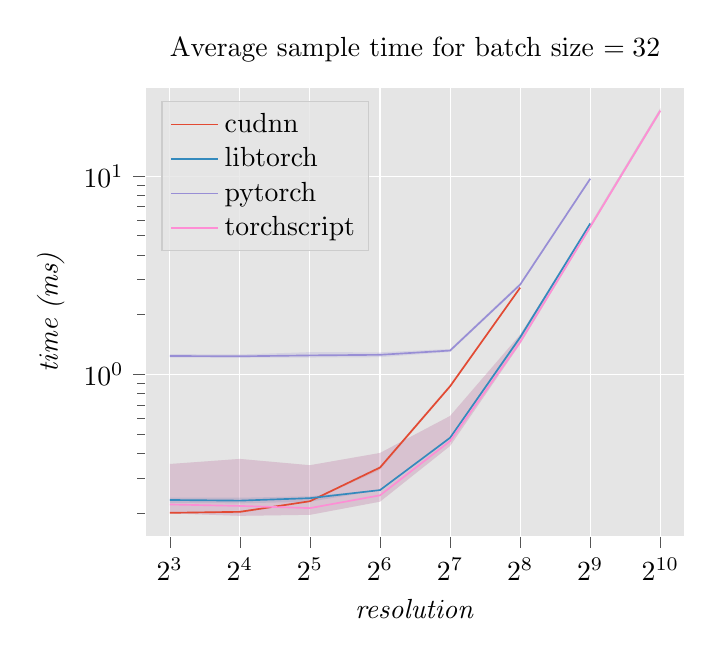
\begin{tikzpicture}

\definecolor{color0}{rgb}{0.886274509803922,0.290196078431373,0.2}
\definecolor{color1}{rgb}{0.203921568627451,0.541176470588235,0.741176470588235}
\definecolor{color2}{rgb}{0.596078431372549,0.556862745098039,0.835294117647059}
\definecolor{color3}{rgb}{0.984313725490196,0.756862745098039,0.368627450980392}
\definecolor{torchscript}{rgb}{0.996078431372549,0.556862745098039,0.835294117647059}

\begin{axis}[
axis background/.style={fill=white!89.8039215686275!black},
axis line style={white},
legend cell align={left},
legend style={fill opacity=0.8, draw opacity=1, text opacity=1, at={(0.03,0.97)}, anchor=north west, draw=white!80!black, fill=white!89.8039215686275!black},
log basis y={10},
tick align=outside,
tick pos=left,
title={Average sample time for batch size $=32$},
x grid style={white},
xlabel={\textit{resolution}},
xmajorgrids,
xmin=2.65, xmax=10.35,
xtick style={color=white!33.3333333333333!black},
y grid style={white},
ylabel={\textit{time (ms)}},
ymajorgrids,
ymin=0.152640394088257, ymax=27.8442975883733,
ymode=log,
ytick style={color=white!33.3333333333333!black},
xticklabels={$2^3$, $2^4$, $2^5$, $2^6$, $2^7$, $2^8$, $2^9$, $2^{10}$},
xtick={3,...,10},
]
\path [fill=color0, fill opacity=0.2, very thin]
(axis cs:3,0.201026)
--(axis cs:3,0.19947)
--(axis cs:4,0.199807)
--(axis cs:5,0.227339)
--(axis cs:6,0.330417)
--(axis cs:7,0.861158)
--(axis cs:8,2.71924)
--(axis cs:8,2.77216)
--(axis cs:8,2.77216)
--(axis cs:7,0.88903)
--(axis cs:6,0.3433)
--(axis cs:5,0.230137)
--(axis cs:4,0.204628)
--(axis cs:3,0.201026)
--cycle;

\path [fill=color1, fill opacity=0.2, very thin]
(axis cs:3,0.239017)
--(axis cs:3,0.224985)
--(axis cs:4,0.223488)
--(axis cs:5,0.227935)
--(axis cs:6,0.260423)
--(axis cs:7,0.475671)
--(axis cs:8,1.50341)
--(axis cs:9,5.67418)
--(axis cs:9,5.86691)
--(axis cs:9,5.86691)
--(axis cs:8,1.56544)
--(axis cs:7,0.483492)
--(axis cs:6,0.261208)
--(axis cs:5,0.242581)
--(axis cs:4,0.238601)
--(axis cs:3,0.239017)
--cycle;

\path [fill=color2, fill opacity=0.2, very thin]
(axis cs:3,1.264947)
--(axis cs:3,1.21564)
--(axis cs:4,1.213545)
--(axis cs:5,1.215587)
--(axis cs:6,1.220171)
--(axis cs:7,1.296469)
--(axis cs:8,2.795173)
--(axis cs:9,9.585992)
--(axis cs:9,9.846071)
--(axis cs:9,9.846071)
--(axis cs:8,2.891976)
--(axis cs:7,1.341868)
--(axis cs:6,1.291262)
--(axis cs:5,1.29437)
--(axis cs:4,1.259168)
--(axis cs:3,1.264947)
--cycle;

\path [fill=white!46.6666666666667!black, fill opacity=0.2, very thin]
(axis cs:3,0.353049)
--(axis cs:3,0.199058)
--(axis cs:4,0.193395)
--(axis cs:5,0.195655)
--(axis cs:6,0.227985)
--(axis cs:7,0.435408)
--(axis cs:8,1.42414)
--(axis cs:9,5.45931)
--(axis cs:10,20.8873)
--(axis cs:10,21.9766)
--(axis cs:10,21.9766)
--(axis cs:9,5.7139)
--(axis cs:8,1.5859)
--(axis cs:7,0.616575)
--(axis cs:6,0.401246)
--(axis cs:5,0.348112)
--(axis cs:4,0.374466)
--(axis cs:3,0.353049)
--cycle;

\path [fill=torchscript, fill opacity=0.2, very thin]
(axis cs:3,0.353049)
--(axis cs:3,0.199058)
--(axis cs:4,0.193395)
--(axis cs:5,0.195655)
--(axis cs:6,0.227985)
--(axis cs:7,0.435408)
--(axis cs:8,1.42414)
--(axis cs:9,5.45931)
--(axis cs:10,20.8873)
--(axis cs:10,21.9766)
--(axis cs:10,21.9766)
--(axis cs:9,5.7139)
--(axis cs:8,1.5859)
--(axis cs:7,0.616575)
--(axis cs:6,0.401246)
--(axis cs:5,0.348112)
--(axis cs:4,0.374466)
--(axis cs:3,0.353049)
--cycle;

\addplot [semithick, color0]
table {%
3 0.200238913297653
4 0.202598989009857
5 0.229123681783676
6 0.338942557573318
7 0.870264947414398
8 2.73578190803528
};
\addlegendentry{cudnn}
\addplot [semithick, color1]
table {%
3 0.232446998357773
4 0.230680495500565
5 0.237425118684769
6 0.260794192552567
7 0.47879546880722
8 1.53802895545959
9 5.7626690864563
};
\addlegendentry{libtorch}
\addplot [semithick, color2]
table {%
3 1.23768603801727
4 1.23296797275543
5 1.24600088596344
6 1.25468814373016
7 1.31825852394104
8 2.83480596542358
9 9.69671154022217
};
\addlegendentry{pytorch}
\addplot [semithick, torchscript]
table {%
3 0.220640391111374
4 0.216945394873619
5 0.211528897285461
6 0.245379000902176
7 0.460912704467773
8 1.45570909976959
9 5.53999090194702
10 21.3651218414307
};
\addlegendentry{torchscript}
\end{axis}

\end{tikzpicture}
